%%% Local Variables: 
%%% mode: latex
%%% TeX-master: "../KanjiHWR"
%%% End: 

\chapter{Technical Design of the Application}
\label{chap:technicaldesign}

The focus of this chapter is on the general architectural choices made during
the development of the system. In this chapter, the technical design aspects 
of the application are described. The general system architecture is layed out in
section~\ref{sec:systemarchitecture}. It contains the global view on the software
architecture in section~\ref{sec:globalarchitecture}, the data flow in within
the system in section~\ref{sec:arch:systemdataflow} and describes the design
of the individual modules in section~\ref{sec:arch:softwaremodules}.
Section~\ref{sec:frameworkanddevices} describes the technical set-up and 
framework choices. However, the handwriting recognition engine is described 
in detail in a separate 
section~(see chapter~\ref{chap:handwritingrecognitionengine}).

\section{System Architecture}
\label{sec:systemarchitecture}

The system architecture of the Kanji Coach follows the requirements of an 
e-learning environment dealing with the specific difficulties for learners 
of the Japanese script (see chapter~\ref{chap:japanasescript}) and those of an 
on-line handwriting recognition. Techniques of handwriting recognition are 
reviewed in chapter~\ref{chap:onlinehwr}. The general requirements of an 
e-learning application are presented in chapter~\ref{chap:elearning}. 
The resulting specific conceptual design choices have been 
layed out in chapter~\ref{chap:conceptualdesignofkanjicoach}. This
section deals with the technical aspects of the system design.

\subsection{Global Architecture}
\label{sec:globalarchitecture}

The global architecture of the application follows the Model-View-Controller
(MVC) design pattern. This paradigm is used as a general model, however, 
it is not implemented the strict way proposed by~\shortcite{Krasner1988}.
Figure~(\ref{fig:modelviewcontroller}) shows the general set-up of the 
MVC design pattern after~\shortcite{Krasner1988}. xxx: Also 
figure~(\ref{fig:modelviewcontroller2}) - decide how it should be done and use
the appropriate gfx. xxx!
In the MVC paradigm the \emph{model} is a domain-specific software, 
an implementation of the central structure of the system. It can be a simple
integer, representing a counter or it could be a higly complex object structure, 
even a whole software module. The \emph{view} represents anything graphical. 
It requests data from the model and displays the result. The \emph{controller} 
is the interface between the model and the view. It controls and scheduls the 
interaction between the input devices, the model and the 
view~\shortcite{Krasner1988}.
%xxx Make this a graphic, not a photographic image of a graphic 
\begin{figure}[htbp]
\begin{center}
\includegraphics[scale=0.5]{images/TechnicalDesign/MVC.png}
\caption{The Model-View-Controller paradigm}
\label{fig:modelviewcontroller}
\end{center}
\end{figure}

%xxx Make this a graphic, not a photographic image of a graphic 
\begin{figure}[htbp]
\begin{center}
\includegraphics[scale=0.5]{images/TechnicalDesign/ModelViewControllerDiagram.png}
\caption{The Model-View-Controller paradigm AGAIN!}
\label{fig:modelviewcontroller2}
\end{center}
\end{figure}

A global overview of the system architecture can be seen in 
figure~(\ref{fig:globalarchitecture}).
%xxx Make this a graphic, not a photographic image of a graphic 
\begin{figure}[htbp]
\begin{center}
\includegraphics[scale=0.5]{images/TechnicalDesign/GlobalArchitecture.png}
\caption{The global architecture of the software system}
\label{fig:globalarchitecture}
\end{center}
\end{figure}

\subsection{System Data Flow}
\label{sec:arch:systemdataflow}
The system data flow is shown in figure~(\ref{fig:systemdataflow}).
%xxx Make this a graphic, not a photographic image of a graphic 
\begin{figure}[htbp]
\begin{center}
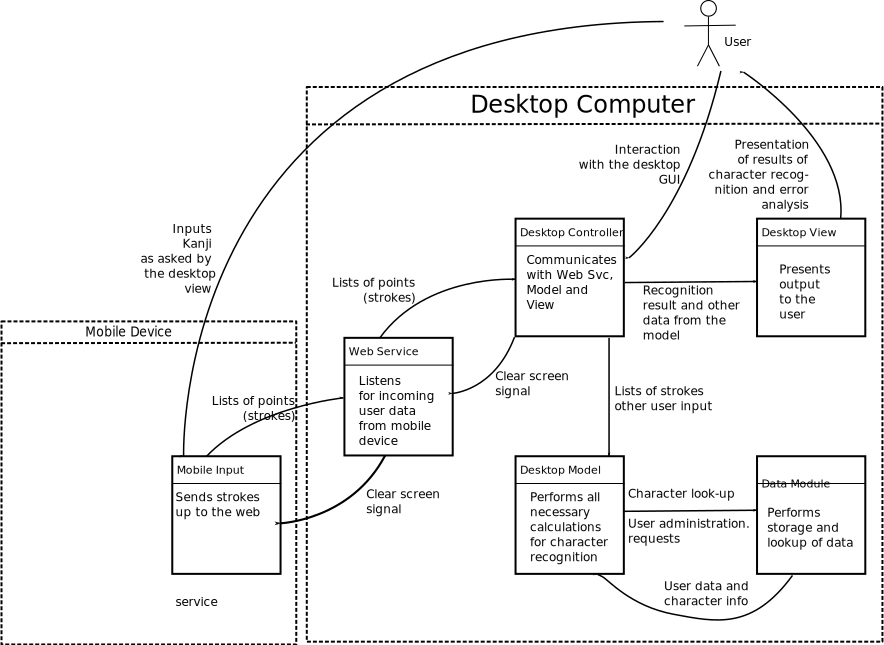
\includegraphics[scale=0.5]{images/TechnicalDesign/SystemDataFlow.png}
\caption{The data flow within the software system}
\label{fig:systemdataflow}
\end{center}
\end{figure}
The controller lies in the centre of the application, it runs on the stationary
device. It contains a web service that is used as an interface to receive data 
from the mobile view. The desktop view is the main interaction point for the 
user. The model contains the logic, while the data access layer provides a 
reusable interface for storing data. 

\subsubsection{Communication}
\label{sec:communication}

The communication between the different parts of the application is realised 
in two independet and distinct ways. The communication between the 
modules running under the same process is realised via a messaging system. 
The communication between the modules that run on different devices
or at least as a separate process is realised via a web service.

\emph{Loose coupling} is used here as a term to emphasize that different modules 
in a larger system are only loosely connected and do not depend largely on each 
other. \emph{Coupling} can be understood as the degree of knowledge a module or 
class have of each another. The lesser the knowledge of each other the software 
modules can manage with, the more loose the coupling.

In the course of the design and development cycles of the Kanji Coach, 
it became apparent that it has to be possible to attach different views, 
input devices and data storage systems to the controller. This is due to the 
distributed nature of the application. 
In order to ensure that the handwriting data input view, which currently runs 
on a mobile device, can run on a different device, it had to be loosly coupled 
to the main controller. Therefore, the communication between the mobile view 
and the main controller is realised via a web service. 
Because of this communication structure, it is possible to exchange the 
handwriting data input view with a different one, for instance when running 
the application on a device like a tablet PC. The implementation of the 
communication structure within the web service is described in greater detail 
in section~\ref{sec:arch:webservice}.

The messaging system that forms the communication structure between the software 
modules running as the same process is realised with a message class that
can be manipulated by the modules using these messages.
Technically, the web service and the controller both run as a subprocess of the 
main desktop view. When the web service receives a request and accompanying data
from the mobile view, both request and data are bundled into an encapsulated
message and passed to the controller. A similar type of message is used for 
requests from the controller to the model, for instance a recognition task that 
needs be performed.

\subsubsection{Recognition Data Flow}
\label{sec:arch:recognitiondataflow}

\subsubsection{Learning Data Flow}
\label{sec:arch:learningdataflow}

\subsection{Software Modules}
\label{sec:arch:softwaremodules}

\subsubsection{Mobile GUI}
\label{sec:arch:mobilegui}

\subsubsection{Desktop GUI}
\label{sec:arch:desktopgui}

\subsubsection{Web Service}
\label{sec:arch:webservice}

http://de.wikipedia.org/wiki/Windows_Communication_Foundation
http://en.wikipedia.org/wiki/Web_service
http://kleineurl.de/1kfd1k.htm


\subsubsection{Recognition Module}
\label{sec:arch:recognitionmodule}

\subsubsection{Learning Module}
\label{sec:arch:learningmodule}

\section{Framework and Devices}
\label{sec:frameworkanddevices}

\subsection{Operating System}
\label{sec:operatingsystem}

\subsection{Framework}
\label{sec:framework}

http://de.wikipedia.org/wiki/Windows_Communication_Foundation

.NET vs. Java etc.

\subsection{Desktop Computer}
\label{sec:desktopcomputer}

\subsection{Pen Input Device}
\label{sec:peninputdevice}

warum mobil? - damit man sehen kann, was man macht!

\subsubsection{Stylus Input}
\label{sec:stylusinput}

